\documentclass[12pt]{article}
\usepackage{svg}
\usepackage{graphicx}
\usepackage{subfig}
\usepackage{float}
\usepackage[margin=1in,includefoot]{geometry}
\usepackage{fancyhdr}
\pagestyle{fancy}
\renewcommand{\footrulewidth}{1pt}

\begin{document}

\begin{titlepage}
	\begin{center}
	\begin{figure}[t]
	\hspace*{0.35cm}
\includegraphics[width=1.0\textwidth]{uclLogo}\\
	\end{figure}
	\line(1,0){300}\\
	[0.25in]
	\huge{\bfseries ArcheoReport}\\
	[2mm]
	\line(1,0){200}\\
	[1.5cm]
	\textsc{\LARGE University College London}\\
	\textsc{\normalsize Department of Computer Science}\\
	\textsc{\normalsize COMP103P Application Project}\\
	\textsc{\normalsize Team38}\\
	[5cm]
	\end{center}
	\begin{flushright}
	{\large Authors: \\}
	Mohammad Hossein Afsharmoqaddam\\
	Varun Mathur
	\end{flushright}
\end{titlepage}
\tableofcontents

\newpage
\section{Abstract}\label{sec:abstract}
Our application project was assigned to the Egyptian Museum of Turin, Italy. We had to develop an exhibition based management tool which would be used by the museum professionals when they are hosting exhibitions outside of their local location. It is essentially an effective tool for museums with archaeological collections.  
\par
The application is designed in such a way where the user is able to create a full ``condition report''  about the state of preservation of the artefacts. ``A condition report'' is a detailed description of the condition of a museum artefact typically produced on the occasion of loans for exhibitions, special handling sessions, packing or restoration projects. 
\par
Additionally, the user is then able to generate a pdf file after filling out the form and save it to their database for further references and creating new forms. To expand, the app has a simple and user friendly interface with various field and dropdown menus and controlled vocabularies and it is able to acquire multiple images of the artefacts. The application allows the user to either upload a photo from the directory of their device or to take a photo from the camera provided on their device. After uploading the photo they are able to annotate the photos using their fingers or a tablet pen. 
\par
Furthermore, the application provides two view screens which are, the ``view forms'' and ``view gallery''. Both of these screens showcase and group their data and the user is able to filter the data by the filtering options provided. 




\newpage
\section{Context}\label{sec:context}

\subsection{Background}
Our team has been in contact with Paolo Del Vesco, a UCL honorary researcher and a curator at the museum and Marco Rossani the registrar of the museum.  The Egyptian Museum of Turin also known as ``Museo delle Antichita'' is the only museum other than the Cairo museum that is dedicated solely to Egyptian art and culture. According to the museums website ``the collections that make up today’s Museum were enlarged by the excavations conducted in Egypt by the Museum’s archaeological mission between 1900 and 1935 (a period when finds were divided between the excavators and Egypt).''

\subsection{Purpose}\label{sec:purpose}
As discussed in the Abstract the museum loans artefacts for exhibitions, have special handling sessions and packing or restoration projects. Therefore, the museum needs to be able to keep track of each artefact and be able to check the artefacts conditions before and after the sessions. 
\par
However, majority of these actions have been paper form based and this application fundamentally will be digitalising the records of the artefacts. By digitalising the system we have brought many advantages which were not possible before in the paper based system which will be discussed below.  

\subsubsection{Easy Access}
From the moment a form is created it becomes accessible from any of the tablets which has the application downloaded. By having a paper based system, a paper file cannot be accessing by another employee at the same time and it is usually housed in file or cabinet which access must be requested.

\subsubsection{Filtering and Searchable Text}
The application allows the user to be able to locate and view forms based on their specific exhibition date and also has a gallery screen which provides all of the photos of the artefacts which can be filtered by the different parameters provided. This is extremely useful since if a client request a form, the museum will be able easily search the form required from their database.

\subsubsection{Cost Savings}
The switch to digitalising a system saves money for many establishments. By having a digitalised system we are minimising the cost of papers, secure file cabinets that the files need to be archived in and adding this to the cost of filing clerks and the downtime required to find specific forms the cost increases substantially.



\newpage
\section{Team Member Summary}

\subsection{Mohammad Hossein Afsharmoqaddam}
Mo did not have any prior android development experience, therefore this was a new area for him to explore. He previously has had experience with C and Java from his university courses and basic web development. He has always liked frontend development and design, therefore his responsibilities were mainly the User Interface elements, navigation and the overall Logic of the application. 

\subsection{Varun Mathur}
Varun has 4 years of Android experience. He has written a few apps as part of summer programs and internships. Varun did a lot of work on the back end functionality of the app, including implementing data persistence and implementing dynamic views that were populated with this data. This consisted of creating classes to represent objects in the system (Reports, Images, Annotations, Defects, Exhibitions), and then implementing the logic to store and retrieve this information and then present this data in the correct views. Additionally, Varun implemented the photo capture and annotation functionality that is present in the app as well as the “filterable” gallery.

\subsection{Rouzbeh Mehregan}





\newpage
\section{Work Plan (GANTT CHART)}
To be as efficient and productive as possible and a Gantt Chart offers many advantages we decided to use this method to enhance our communication, and to be able to see our project over the long term and to track the results of each task. 
\par
In a glance we were able to keep track of incoming tasks, and tasks that remained to be completed, therefore we avoided any completion confusion. Furthermore, by being able to look ahead we were able to effectively allocate resources and tasks to each member. 

\begin{figure}[h]
\begin{center}
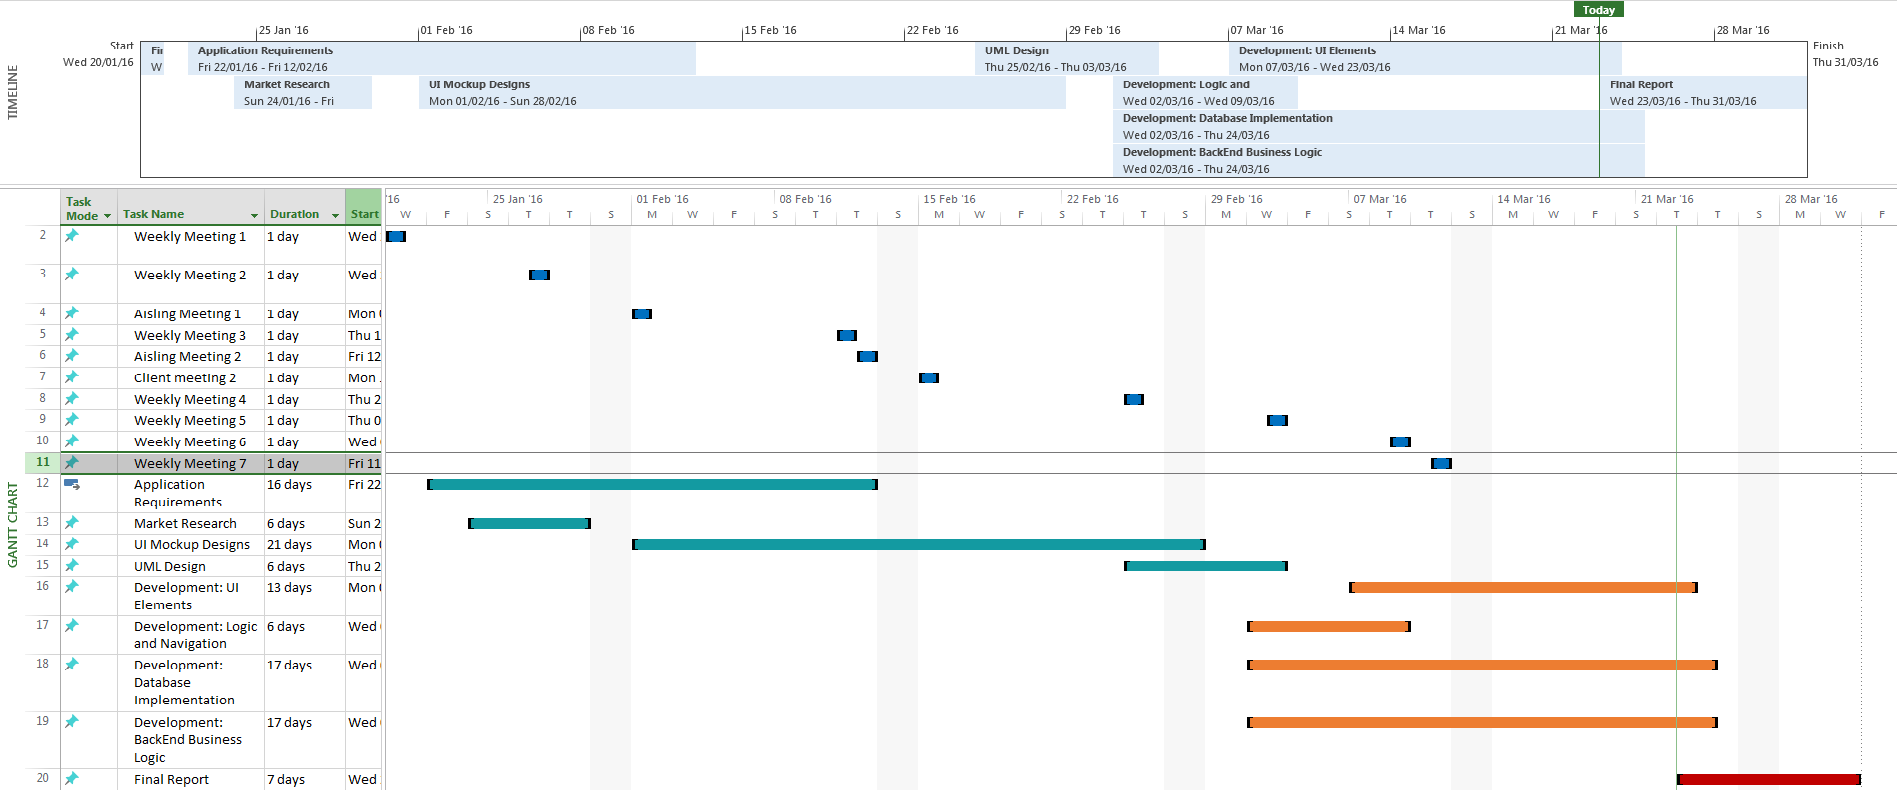
\includegraphics[width=1.0\textwidth]{ArcheoReportGantt}
\end{center}
\end{figure}

As you can see from the figure, we separated the project into three different areas. The blue colour reprsents our team meetings during the project, the turquoise colour represents the timeline of our early planning, requirements and mock-up stages. The orange colour represents our development and programming phase and the red colour represents the evaluation and the creation of the final report. Additionally, the timeline on top of the chart provides us with the exact duration that each task should be completed. 

\newpage
\section{Requirements}
\subsection{Project Brief}
Our brief was to design an app for the UCL Institute of Archeaology that would enable them to generate condition reports for artefacts using a tablet app. Additonally, they wanted some additionally functionality including photo capture and annotation, auto completion of data fields using information from Excel files and signature authentication. We were given these specifications by the client in our initial meeting. After this we took all of their requirements for the app and prioritised them based on a cost/necessity basis. Essentially requirements were ranked based on their necessity versus cost of implementation. When we finished we showed our analysis to the clients who then suggested changes. Finally we ended up with a completed MoSCoW analysis of the requirements.

\subsection{MoSCoW Requirements}
\subsubsection{Must Have}
\begin{description}
\item [Report Generation - (PDF Generation)]
Condition reports for artefacts must be output by the app in PDF format. The format and contents of the report should be identical to the current form.

\item [Report Data Should Be Saved for Subsequent Reports]
The client said that when an item is moved into an exhibition, a condition report is generated. Then after the exhibition another report is done, with reference to the prior one.

\item [Condition Reports Must Be Grouped by Exhibition]
This entails a higher level menu wherein the user can create and manage exhibitions. Then within the context of one exhibition the user can manage condition reports.

\item [Image Selection Wizard Screen]
When the user chooses to add a photo to a report, the menu should allow them to choose images from file directory or capture and annotate a new photo. Additionally, user should be able to mark a photo as a packing photo.

\item [Photo Capture]
The app must allow the user to take photos of artefacts. These photos should be stored for later reference. Most likely cloud storage.

\item [Photo Annotation]
The app must facilitate annotating images to mark defects on artefacts. These annotations must be classified, and linked to a textual description. 

\item [Auto-Fill Form]
The text inputs on the form will fill themselves in from data stored in an excel file once the user types in an item’s inventory number. 

\item [Storage of Descriptions for Annotations - Links to Visual Annotations]
Images will have to be categorised by their defects, thus annotations will have concrete classifications. Additionally, annotations will be linked to textual descriptions of the defect.

\item [Picture Browsing with Defect Classification]
Pictures will be classified based on defects present in them. User must be able to search a gallery of images, and search by defect.

\item [Import Excel data]
The user should be able to import data in the form of an excel document. This data will be used to auto complete fields in the condition report form. 

\end{description}

\subsubsection{Should Have}
\begin{description}
\item [Zooming functionality on annotation drawing screen]
User should be able to zoom in while drawing annotations such that they can draw with greater detail and precision.
\end{description}
\subsubsection{Could Have}
\begin{description}
\item [Signature]
The user could sign off on reports using the tablet in order to verify and authenticate their identity.

\item [Login/Identification (Could replace signature)]
As an alternative to signatures, users could sign in using a username and password to verify identity. Also enhances security as users will have to be logged in to use the app.

\item [Printing]
Printing condition reports is another feature that could be implemented. Android has this functionality.
\end{description}
\subsubsection{Will Not Have}


\subsection{Glossary / Data Dictionary}
\begin{description}
\item [Condition Report] The clients currently conduct condition reports on museum artefacts in transit. In these reports, they record information about the condition of the artefact including any \textbf{defects} that are present. Additionally they note information about the way the item has been packed as well as general information about the artefact itself. Artefacts are identified using their inventory number which is stored in the report

\item [Exhibition] The clients would like to group their reports by exhibition. That is, the exhibition that the artefact is in transit to/from. Each exhibition has the following information: Name, Location, Start Date, and End Date.

\item [Defect] The clients have a set list of defects which they try to identify and record when doing condition reports on artefacts. In the context of the app, the user must be able to select defects from a pre set list when creating a condition report.

\item [Annotation] The clients wanted to be able to draw annotations on photos of artefacts and associate an annotation with a specific defect and then have those annotated photos saved on the device. In this case, annotations are just drawings, but they must be linked to a defect. Additionally, an annotated image must store the defects that are associated with the annotations on the images. This way, in the gallery section of the app, photos may be filtered by the defect that they depict. 
\end{description}

\section{Design}
\subsection{Rationale for Using the Model-View-Controller Framework}
We decided to follow an MVC approach to the solution for a variety of reasons. First, Android applications are programmed in JAVA, an object oriented programming language. Moreover, due to the nature of our requirements an object oriented approach suited our solution. Based on our analysis and understanding of the application brief we translated 3 real world objects into JAVA classes: Reports, Exhibitions, and Annotated Images. These objects would be the models in the MVC framework.\\

Android development lends itself to the MVC framework in that Views are created using XML, and then populated with information from Models through Activity classes. Thus in this case, we would create are views using XML, and then have Activities work as the controllers in the system, handling user input and managing the exchange of information between model and view and vice versa. 
\subsection{Models}
\subsubsection{Exhibition Class}
Due to the nature of our clients' work, all condition reports are conducted within the context of an exhibition. In the app, this would be reflected in the user interface, as all condition reports would be generated within the higher context of an exhibition. Thus we created an exhbition class in order to store information about specific exhbitions including: the name, the location, and the start and end dates of the exhibition.
\subsubsection{Report Class}
The report class maintains all of the information from a single condition report conducted on a single artefact. The report therefore must encapsulate every bit of information that is entered from the condition report generation screen. Moreover, the report class contains a reference to an exhibition object which is its contextual exhibition.
\subsubsection{Annotated Image Class}
One of the clients' most important requirements was to be able to capture photos of artefacts and then annotate the photos to illustrate defects in the item. Photo capture and annotation would be done under the context of a specific condition report (i.e. the user would capture and annotate photos of the artefact while conducting the condition report on the same item). Thus these images would have to be linked somehow to the report. Moreover, the annotations would be linked to defects, and these defects would have to be stored along with the image. This warranted the creation of an AnnotatedImage class which contains a list of defects, a reference to its contextual report, and a file path to the image itself on the device.

\subsubsection{UML Class Diagram}

  \includegraphics{archeoreportuml.png}

\subsection{Views}
The user must be able to both create and view models in the system. Thus we reasoned that views could be generally split into two categories: \textit{viewers} and \textit{creators}. Thus in our implementation, each model has an associated \textit{viewer} and \textit{controller}. The role of a  \textit{viewer} view is to display information from a model or models to the user, while a \textit{creator} view provides all the user input elements to allow for the construction of a model. All views have associated controllers which either bind data from the model to populate the view, or handle user input and take that data to create a model.


\subsubsection{Viewers}
\label{sec:Viewers}
\textit{See appendix for user interface mockups}
\paragraph{Exhibition Viewer}
This was the highest level screen. Exhibition objects are loaded from the database and passed into a ListView. Each ListItem displays the name, location, and dates of each exhibition. Clicking on an exhibition in the list leads to the ``Report Viewer'' screen with the exhibition passed as context.

\paragraph{Report Viewer}
This screen loads up Reports from the database under the context of the higher level exhibition. This is achieved using a simple database query (explained in Persistance section). The reports are loaded into a ListView. Each item displays the inventory number of the artefact and the date the report was created. Clicking on a report will open the corresponding PDF of the report in the device's native document viewer.

\paragraph{Image Viewer (Gallery)}
This screen presents the user with a grid of annotated images loaded from the device. Clicking an image will open it full screen in the device's native image viewer. The user can also choose to filter images by Exhibition, Report and Defect. This is achieved once again using database queries. Once the correct AnnotatedImage objects are loaded, their file paths are lazily loaded into an ImageView in each GridItem so as not to slow down the interface. 

\subsubsection{Creators}
\label{sec:creators}

\paragraph{Exhibition Creator}
View with 4 input elements to allow the user to create an Exhibition object.

\paragraph{Report Creator}
Replication of the paper condition report form. Full page view with inputs for all the fields of a condition report, allowing the user to create Report objects. Additionally, this view had a button which allowed the user to attach photos to the report. Adding an image would give the option to annotate it and thus lead the user to a view where they could ``create'' an annotated image.

\paragraph{Annotated Image Creator}
This view allowed the user to annotate images from the device or from the camera. The user is presented with some options to change brush width and colour. Additionally, the user can select which defect they want to associate with their annotations. When the user is finished, the result is a new Annotated Image object which is saved on the device. \\

In order to achieve the annotation functionality a custom class was created, extending Android's native ImageView. This new class, called AnnotationView dsiplays an image and detects user touches to draw annotatations on top of the image. The annotated photo can be obtained in Bitmap form by retrieving the object's drawing cache. 



\subsubsection{Controllers}
\label{sec:Controllers}

In this system, controllers were implemented as Android Activities. The Activity class in the Android environment encapsulates a user's interactions with a single view. Thus each view in the system has an associated Activity which it is bound to. Within each Activity lies the logic which binds data to elements in the view, or generates and updates models from data input in the user interface. Additionally, the Activity is responsible for actions like generating PDF documents, saving annotated images to file, and updating views based on user input. 

\paragraph{Specific Implementation Details}
PDF generation was achieved using the built-in PDFDocument API present in the Android SDK. In the CreateReport Activity, upon report completion a new Report object is generated with the input data. This object is then passed to a method which generates the PDF version of the report. This is achieved by creating a containing view object (a LinearLayout) and then adding TextViews containing textual data from the report as children to this container. Additionally, a maximum of 4 ImageViews are added to the container and supplied with Annotated Images from the report. Everytime a view is added to the container, its coordinates must be specified such that they fit into the 595 x 842 (A4 size) canvas. Then the LinearLayout is ``drawn'' onto the canvas of a PDFDocument object, and the corresponding PDF file is saved onto the device's external storage in the directory: \textit{ArcheoReport/Reports/<Exhibition Name>/<Report Inventory Number>.pdf} \\

In the image annotation Activity, the controller logic is responsible for responding to user input and changing the parameters of the annotations. There are three parameters for the annotation view: annotation color, annotation size, and defect classification. The controller listens for input on these menus and then updates the AnnotationView to change the parameters. Additionally, there is an ``eraser'' button. When this is toggled, the controller updates the AnnotationView to erase annotations rather than draw new ones. When the user finishes the annotation, the annotated images in saved to file in the following directory: \textit{ArcheoReport/Images/<Exhibition Name>/<Report Inventory Number>\_annotated\_<timestamp>.pdf} \\


\subsubsection{Model Persistance}
A key part of the implementation was saving objects in the database when they were created so that they could be loaded and presented to the user in the interface. Android has built-in database functionality: there is an API to allow the programmer to store data in an SQLite database. Initially we were going to use this API to store the objects in the application. However, we found a third party library called SugarORM which vastly simplified this process. SugarORM works as follows: Objects which are to be persisted must extend the ``SugarRecord'' class. Then when an object is created, ``SugarRecord.save()'' must be called on the object to save the object in the database. The library saves all instance variables of the object in a row of a table named after the class. Thus the programmer is completely removed from the process of actually interacting with the database. Database queries can also be conducted on these tables, with references to the members of the class. Additionally, each object is assigned a unique ID which can be used to retreive it from the database. Queries will return \textit{Plain Old JAVA Objects} which can then be used right away in the application.

\section{Testing and Installation}
Our development schedule was iterative and driven by producing protoypes at various milestones. We resolved to create a protoype which met all the requirements to a standard that we were satisfied with. Then we sent it to the client to get their feedback. Then began a cycle where we would implement their feedback, send them a new build and continuously fine tune the application to the point where the client was satisfied. \\

The reason we did this was because our development time was limited and so was our manpower. We decided that the fastest way to create a working product would be to follow a development schedule that emphasised building partially complete, but running prototypes and getting as much feedback from the client as we could, as often as we could. Each build would introduce a new feature or small set of features that the client could test and evaluate, then they would tell what to change. We would change it, add more features and repeat the process. This way we minimised the time spent implementing features the wrong way. \\

Each prototype would be tested by us before sending it to the client. Because each prototype typically introduced a small set of new features, testing on each incremental build consisted of testing that the new feature worked and integrated well with the rest of the app. Once testing was complete, we would send the new build to the client via email. 

\section{Status \& Evaluation}
\subsection{Work Completed}
Looking back to our project, we believe we have completed all of the fundamental and key functionalities that our clients had asked for and more. During the development of the application we have been constantly in touch with our clients and using their feedback to continuously improve our product. This proved difficult at first as our clients were located in Italy however through different methods of communicating such as skype sessions for important overviews and emails for frequent and minor updates we managed to effectively communicate with our clients. 

\par
We have manged to complete all of our ``must have" requirements. The most difficult requirements were importing an excel file into the system directly therefore we came up with a solution of only importing the csv file which the client agreed to as they already have the csv files of their forms in their database. Furthermore, generating a pdf file proved difficult at first as they were very minor details that we had to consider when implementing to get the desired results, however we managed to find the correct library and documentation to solve the problem.

\par
The ``should have" part of our MoSCow analysis has been changed throughout the development series. After many meetings with the clients they decided they did not need many of the features needed. For example there was no need of any authentication as the application will be only available to the trusted employees of the museum and no one else will have access to the application. Moreover they decided having signatures on the condition reports for the artefacts were redundant and did not add much purpose for the functionality they needed. Finally, a printing functionality from the application was not needed as the whole purpose of this project was to digitalise their system, however they have the ability to transfer the generated pdf files onto computers for printing if needed.

\subsection{Risks}
Risk management is a critical matter and below we will be going over a few risks within our scope of our project and how we managed to minimise and solve each of them accordingly. 

\subsubsection{Risk 1: Exclusivity of project}
Within software development it is inherently difficult to create a completely new and unique design given the amount of applications being used worldwide. To minimise any plagiarism or replication of any other software and their design we communicated with our clients very frequently to work out exactly how they wanted the app to look like and what features they were interested in for our team to implement. 

\subsubsection{Risk 2: Requirements Inflation}
As the project moves forward and the development phase begins it becomes apparent that requirements and specification is incomplete or it contains conflicting themes. We minimised this risk happening as we were taking an agile approach. Within an agile approach we utilised the concept of an ambassador user, in our case the team leader to be readily available to answer any of the client’s questions and make trade-off decisions on the project. As well as this approach we tried our best to confirm and finalise the core requirements in the beginning of the development phase to avoid any future obstacles. 

\subsubsection{Risk 3: Compromising on designs and planning stage}
For many developers in order to get stuck in with the ``real task", the design and planning stage is either skipped or poorly done. This can have huge downtime in the long-term and can cause many problems throughout the life time of the project. Therefore knowing this we spent a fair amount of time in our planning phase where we identified the core requirements, created a high level design of the project and created mock-ups of the UI design and implemented Unified Modelling Language. This phase of planning is apparent as shown in GANTT CHART previously and it has helped us to develop the project as smoothly as possible by minimising the complications and efficiently spending time in the development phase. 

\subsubsection{Risk 4: Gold plating}
Developers sometimes like to spend a lot of time in the beginning creating unnecessary features or making a screen look very stylish. As it is very important to have a very good UI design it is not the most important piece of the application. We detected this risk by finishing all the core and fundamental functionalities of the application and then focusing on the UI design and any other nice to have features. Especially since our client was very much focused on the output and usability of the application rather than how it looked visually. 

\subsection{Final Evaluation}
In conclusion we believe we have created a good user friendly application for the Egyptian Museum of Turin, Italy. Even though one of our team members did not contribute to any of the tasks within this project we still managed to finish the application in the small time frame provided with all of its core features working competently. Additionally, by taking an agile approach we tried to minimise all of the risks presented throughout the project and communicated effectively with each other and to the client to create the best application we possibly could. 


\newpage
\section{Refrences}


\newpage
\section{Appendices}
\subsection{Bi-Weekly Reports}
Written records of our meetings during the phase of the project.

\subsubsection{Report \#1}
 \textbf{Summary Meeting 1 - Mo and Varun - 20/01/2016} 
\par
	Our first meeting was 20th Jan. We met to discuss our initial understanding of the requirements given to us by the client. We wrote up questions that we would ask the client in order to clear up any misunderstandings we might have had with the requirements. 
\par
\bigskip	
	\textbf{Client Meeting - Mo and Varun 20/01/2016}
\par
On the same day, we had our first Skype conference with the client. First, they explained the purpose of the application and how and by it would be used. They gave us a more specific list of requirements that they definitely wanted in the app as well as some features that were desirable but not necessary. Furthermore, they were able to answer some of our questions, however some we left unanswered. We resolved to send them an email in order to clarify some details of the application that were still unclear to us. 
\par
\bigskip	
	\textbf{Meeting 2 - Mo and Varun 27/01/2016}
\par
	We had a second team meeting on the 27th of Jan. Based on the requirements that were given to us during the Skype call, we conducted a MoSCoW analysis in which we prioritised the different features of the application. We also drafted and sent an email in which we asked the client for some more information about specific aspects of the application. These included the transfer and storage of information to the museum database, user authentication, and the version of Android they were running. 
\par
\bigskip	
	\textbf{Meeting with Aisling - Mo and Varun 01/02/2016} 
\par
	On 1st Feb, we had our first meeting with Aisling. During the meeting we explained to her our project, the requirements given to us by the client, and the progress we had made so far. Aisling advised us to start making basic mockups of the UI to show the client so that we do not waste time making changes later. She also advised us to consult a technical TA to gauge the difficulty of implementing certain features, namely drawing annotations on pictures in the app. She stressed that it would be unwise to invest too much time into programming anything until we had a solid idea of what the client wants.
\par
\bigskip
	\textbf{Meeting 3 - Mo and Varun 11/02/2016} 
\par
In this meeting we compared our rough ideas for the UI and UX of the app. We drew sketches of the various screens of the app and how they would be linked. We also talked about the kind of ‘workflows’ that the user would experience in the app (i.e. report creation, report viewing, gallery viewing etc.). After discussion, we combined our ideas and began work on a more professional UI mockup using a tool called FluidUI.
After working on this mockup, we realised that there were elements of the app that we were still unsure about. Therefore we resolved to contact our client as soon as possible to discuss these specifics. 
\par
\bigskip

\textbf{Tasks Completed:}
\begin{itemize} 
\item Initial contact with client
\item Consultation with client, clarification of specifications
\item MoSCoW analysis of requirements
\item Research into apps with similar features
\item Storyboarding / UI Mockup
\end{itemize}

\bigskip
We feel that the project is running on time. The client is happy so far and we have had good communication. We are confident in the app’s specifications and we feel that they are realistic and achievable. We feel that we will be ready to start development after reading week.
Plan for Coming Weeks:
	Our plan is to approach development slowly. We will refine our UI mockups and share them with the client to ensure that we have all features and screens included in our design.
	Then we will start to plan development. We will identify all the components that need to be implemented (i.e. JAVA classes, UI elements, documentation). And we will try to estimate how long these components will take to create, test and install.

\bigskip
	
\textbf{Tasks worked on: Mo Afsharmoqaddam}
\begin{itemize}
\item Being involved in the first Skype meeting with the clients and coming up with questions and clarifying requirements. 
\item Revising the requirements mentioned by the client and trying to come up with a finalised requirements list and sharing/discussing it with the team
\item Creating a MoSCow analysis form with team-mates and researching application with similar functionalities
\item Creating a rough high level mock UI of the functionality of the application on paper and comparing it to the other designs created by team-mates. 
\end{itemize}

\bigskip

\textbf{Tasks worked on: Varun Mathur}
\begin{itemize}
\item Arranged meetings as team leader
\item Met with client, discussed app requirements and specifications.
\item Met with team to discuss requirements, and categorised them using MoSCoW analysis.
\item Did a rough sketch of the app, then met with team mates where we shared our UI ideas
Combined ideas and did a more professional UI mockup on fluidUI
\item Began planning development phase
\item Started research into development platform and planning how we will achieve certain requirements.
\end{itemize}

\subsubsection{Report \#2}
	\textbf{Meeting with Aisling - Mo and Varun 12/02/2016}
\par
	In this meeting, Aisling recommended that we finish our mockups and our MoSCoW requirements and share these with the client. She said that by the end of reading week we should be completely confident in our knowledge of the client’s requirements.
\par
\bigskip
	\textbf{Client Meeting - Varun 15/02/2016}
\par
	In this meeting with the client, we discussed the MoSCoW analysis of the requirements that we had done. Additionally, we shared with them a preliminary mockup of one of the main screens of the app. The client suggested a few changes and we have updated our requirements document to reflect this. We are also working on updating the mockups and creating a complete and finalised mockup. We are planning to complete this and show it to the client on the 28th. 
\par
\bigskip
	\textbf{Meeting with TA- Varun and Rouzbeh 16/02/2016}
\par
We Skyped our teaching assistant and shared with her our progress so far. She said that we were on track and recommended finalising our plans and beginning development. She also suggested an “agile” development approach wherein we develop many iterations of the app and continually improve it until the client is satisfied. 
\par
\bigskip
\textbf{Team Meeting- Mo and Varun 25/02/2016}
\par
	We split up the task of creating final mockups which we hope to finish by the 28th. By the end of next week we plan to finish UML diagrams to aid us later in development. Additionally we have sent the final requirements document to the client for their confirmation. We are now starting to set up for development. We created a Github repository where we will collaborate on the app itself. We also created a Trello page for our team to track tasks for development and also general planning and communication. 
\par
\bigskip

\textbf{Tasks Completed:}
\begin{itemize}
\item Finalised requirements
\item  Presented Mockup
\item  Setup Trello and Github repo
\item  Began planning for development
\end{itemize}
\bigskip

\textbf{Plan for Coming Weeks:}
\begin{itemize}
\item  Get confirmation of our finalised requirements from the clients by Monday Feb 29th.
\item  Finish the UI mockups by Monday Feb 29th and email the client and get their confirmation.
\item  Finish a full UML diagram of the application by Friday March 4th. 
\item  Split up development tasks between members by next week. 
\end{itemize}
\bigskip

\textbf{Tasks worked on: Mo Afsharmoqaddam}
\begin{itemize}
\item Attended meeting with Aisling to report about our progress on our client requirements and mockups design.
\item Creating finalised UI mockups 
\item Started researching Android Studio and the Java language and downloading the required software
\item Started researching on a few requirement criteria of our MoSCow requirements. 
\end{itemize}
\bigskip

\textbf{Tasks worked on: Varun Mathur}
\begin{itemize}
\item Attended Meeting with Aisling
\item Skyped with client to finalise requirements and get feedback on mockup
\item Had Skype call with TA to discuss progress and plans
\item Started work on final mock ups
\item Organised plans to start planning for development by creating UML diagrams for solution
\item Set up Trello for organisation and task management
\item Created Github repo for team
\end{itemize}

\subsubsection{Report \#3}
\textbf{Team Meeting - Mo and Varun - 03/03/2016}
\par
	We worked on mockups to show to the client and also to aid us in development. We also made a UML diagram to map out the system and also help us with development. We are spending a lot of time planning and design, heeding advice given to us early on in the program. We will start on development once we have solid plan and designs that we have 100\% confidence in. This will make development faster because we won’t have to change anything or add new, unexpected features. 
\par
\bigskip
	
	\textbf{Meeting with TA - Mo and Varun 08/03/2016}
\par
We met with our TA, Manal. She told us to quickly get on with development so that we could have something to show to the client. She advocated an iterative kind of development where we made prototypes often and to show to the client and get feedback. She also emphasised a few deadlines in the future we should aim for so that we are not left behind. 
\par
\bigskip	
	\textbf{Team Meeting - Mo and Varun 09/03/2016}
\par
	During this meeting we worked together on our prototype. We divided the tasks between us and we hope to have this done by Monday and show it to the client to get their feedback.
\par
\bigskip
	\textbf{Team Meeting - Mo and Varun 11/03/2016}
\par
\bigskip
	Again we worked on our prototype. No difficulties so far. Components are proving to be less difficult than anticipated. General workflow so far has been: Mo works on UI elements and logic and then Varun implements backend business logic and links views together. 
\par 
\bigskip

\textbf{Tasks Completed:}
\begin{itemize}
\item Finished planning and design
\item Began work and made significant progress on prototype.
\item Met with our TA
\end{itemize}
\par
\bigskip

We were a bit behind in schedule but we have picked up the slack and we feel we are now back on track. We are confident that we can deliver a very good product soon. 

\par
\bigskip

\textbf{Plan for Coming Weeks:}
\par
	Our plan is to deliver a prototype next week. Then we will continually improve on this until the client is satisfied and all requirements are met adequately. Furthermore, after receiving an email from the client we will continue to adjust our design based on their requirements. 
\par
\bigskip
	
\textbf{Tasks worked on: Mo Afsharmoqaddam}
\begin{itemize}
\item Finished finalized mockups
\item Started programming the navigation page, including buttons and navigation drawer
\item Created the most of the structure of the application, and implementing features such as adding/storing data and adding images
\item Created first draft of the report screen
\item Started implementing some UI design
\end{itemize}
\bigskip

\textbf{Tasks worked on: Varun Mathur}
\begin{itemize}
\item Finished Mockups
\item Did significant work on prototype
\item Designed UI elements
\item Implemented database and business logic
\item Implemented annotation functionality
\end{itemize}

\subsubsection{Report \#4}
\textbf{Team Meeting - Mo and Varun - 15/03/2016}
\par
	Continued work on app development. We updated each other on our individual progress. Mo had made updates to the UI, while Varun had implemented the photo capture functionality and database integration.
\par
\bigskip
	
	\textbf{Team Meeting - Mo and Varun 17/03/2016}
\par
Again we updated each other on our progress. Varun had finally got the database integration fully working. Exhibitions and reports could be created and saved to the database. Additionally, PDFs were now being generated when the user created a report. The next step would be getting the image capture and annotation to link up with reports in the database.
\par
\bigskip	
	\textbf{Team Meeting - Mo and Varun 22/03/2016}
\par
	Met to once again update each other on progress. Varun had implemented image capture and annotation, now these images were being saved on the device and in the database. Next step is to create a gallery screen and allow user to filter images by defect, report and exhibition.
\par
\bigskip

	\textbf{Team Meeting - Mo and Varun 24/03/2016}
\par
	Varun has implemented the gallery screen as well as the CSV import functionality. App is functionally complete and meets most requirements. Next step is to implement asthetic improvements and minor functionality improvements. Additionally, code must be cleaned up, documented and generally made more readable to ease maintenance down the line. 
\par
\bigskip

\textbf{Tasks Completed:}
\begin{itemize}
\item Finished a version of final app.
\end{itemize}
\par
\bigskip
	 After having been behind earlier, we picked up the pace and implemented a working version of the app. The app meets specification, must there is room for improvement. The team is happy with what we have achieved given earlier setbacks and our late start. 
\par
\bigskip
\textbf{Plan for Coming Weeks:}
\par
	 Our plan now is to make improvements to the aesthetics and user experience in the app. Additionally we can implement more features that the client wanted but deemed not crucial. We must also work on making the app more extensible by making the codebase more readable and creating documentation. 
\par
\bigskip
	
\textbf{Tasks worked on: Mo Afsharmoqaddam}
\begin{itemize}
\item Worked on some UI elements of the list view
\item Created the Form screen
\item Started writing the final report:
\item Abstract and Background completed
\item Team summary completed
\item Created Gantt Chart and Requirements page completed
\end{itemize}
\bigskip

\textbf{ Tasks worked on: Varun Mathur}
\begin{itemize}
\item Implemented core functionality of app
\item Creating models of objects in the system
\item Data persistence in database
\item Populating views with data from database
\item Image capture and annotation
\item Saving images in database and linking them to specific defects
\item Created gallery screen to allow user to view annotated images and filter by defect, report, and exhibition.
\end{itemize}

\section{User Interface Mockups}

\begin{figure}
  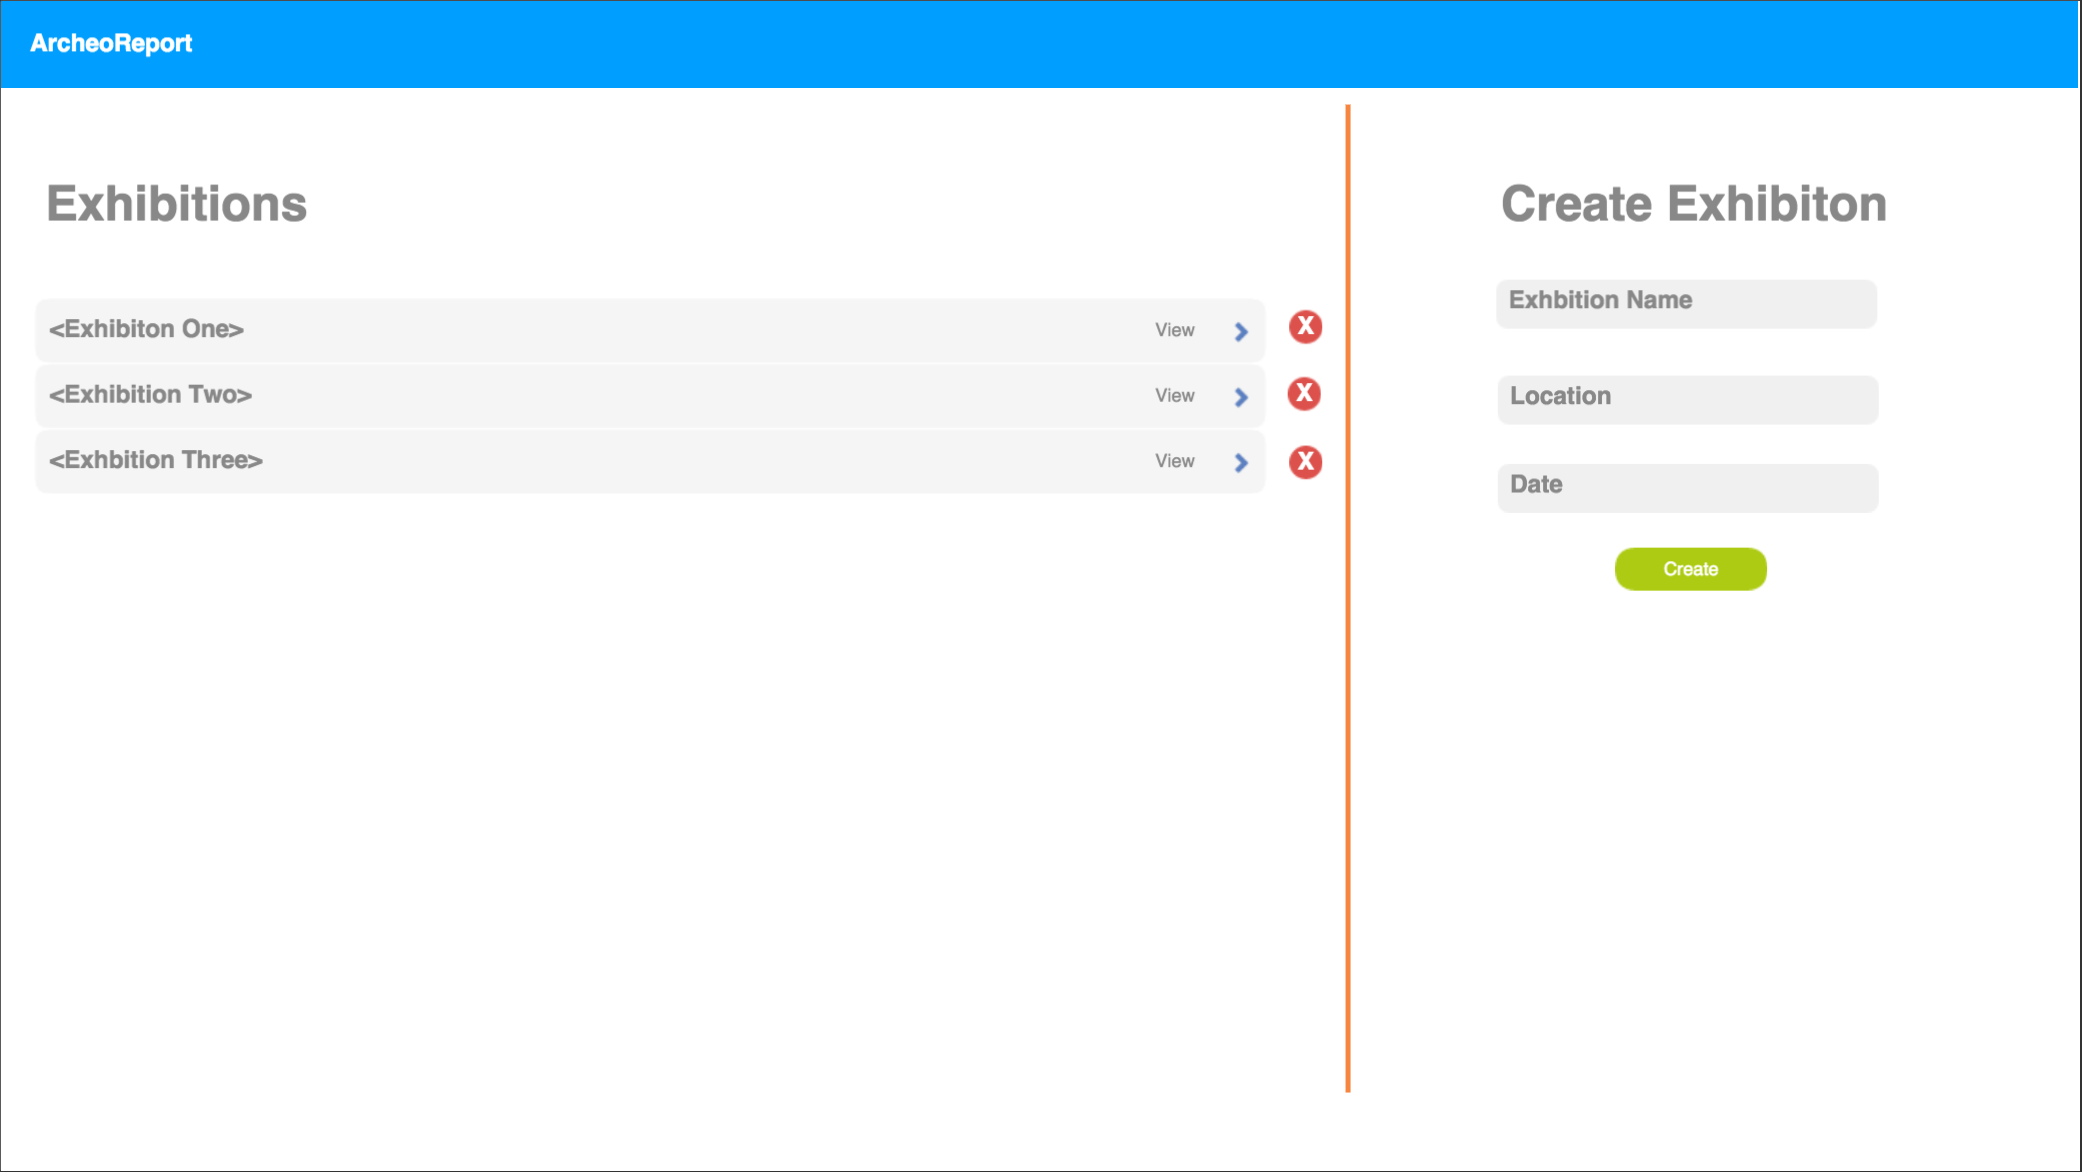
\includegraphics[scale=0.5]{mockup1.png}
\end{figure}
\begin{figure}
  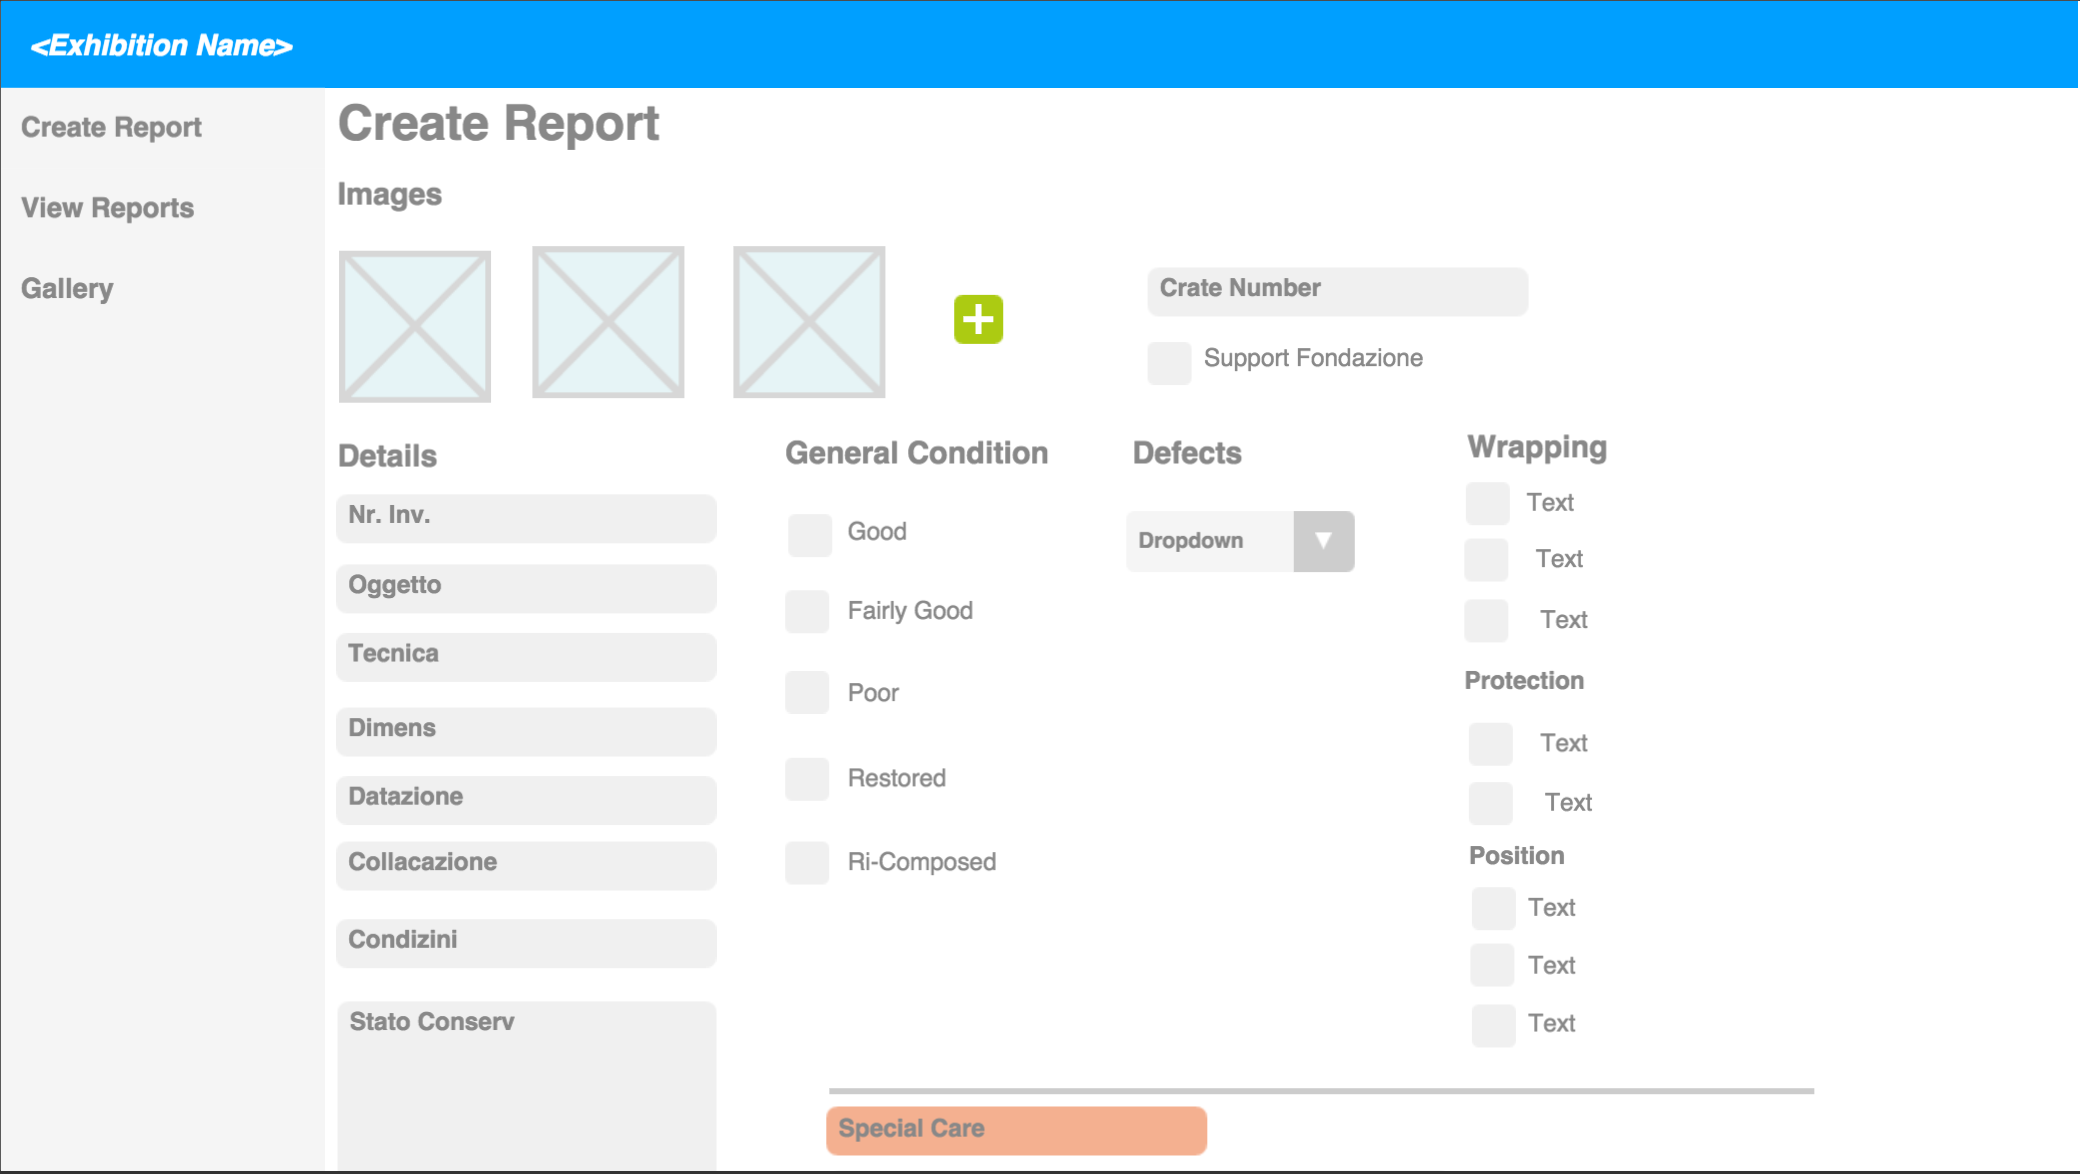
\includegraphics[scale=0.5]{mockup2.png}
\end{figure}
\begin{figure}
  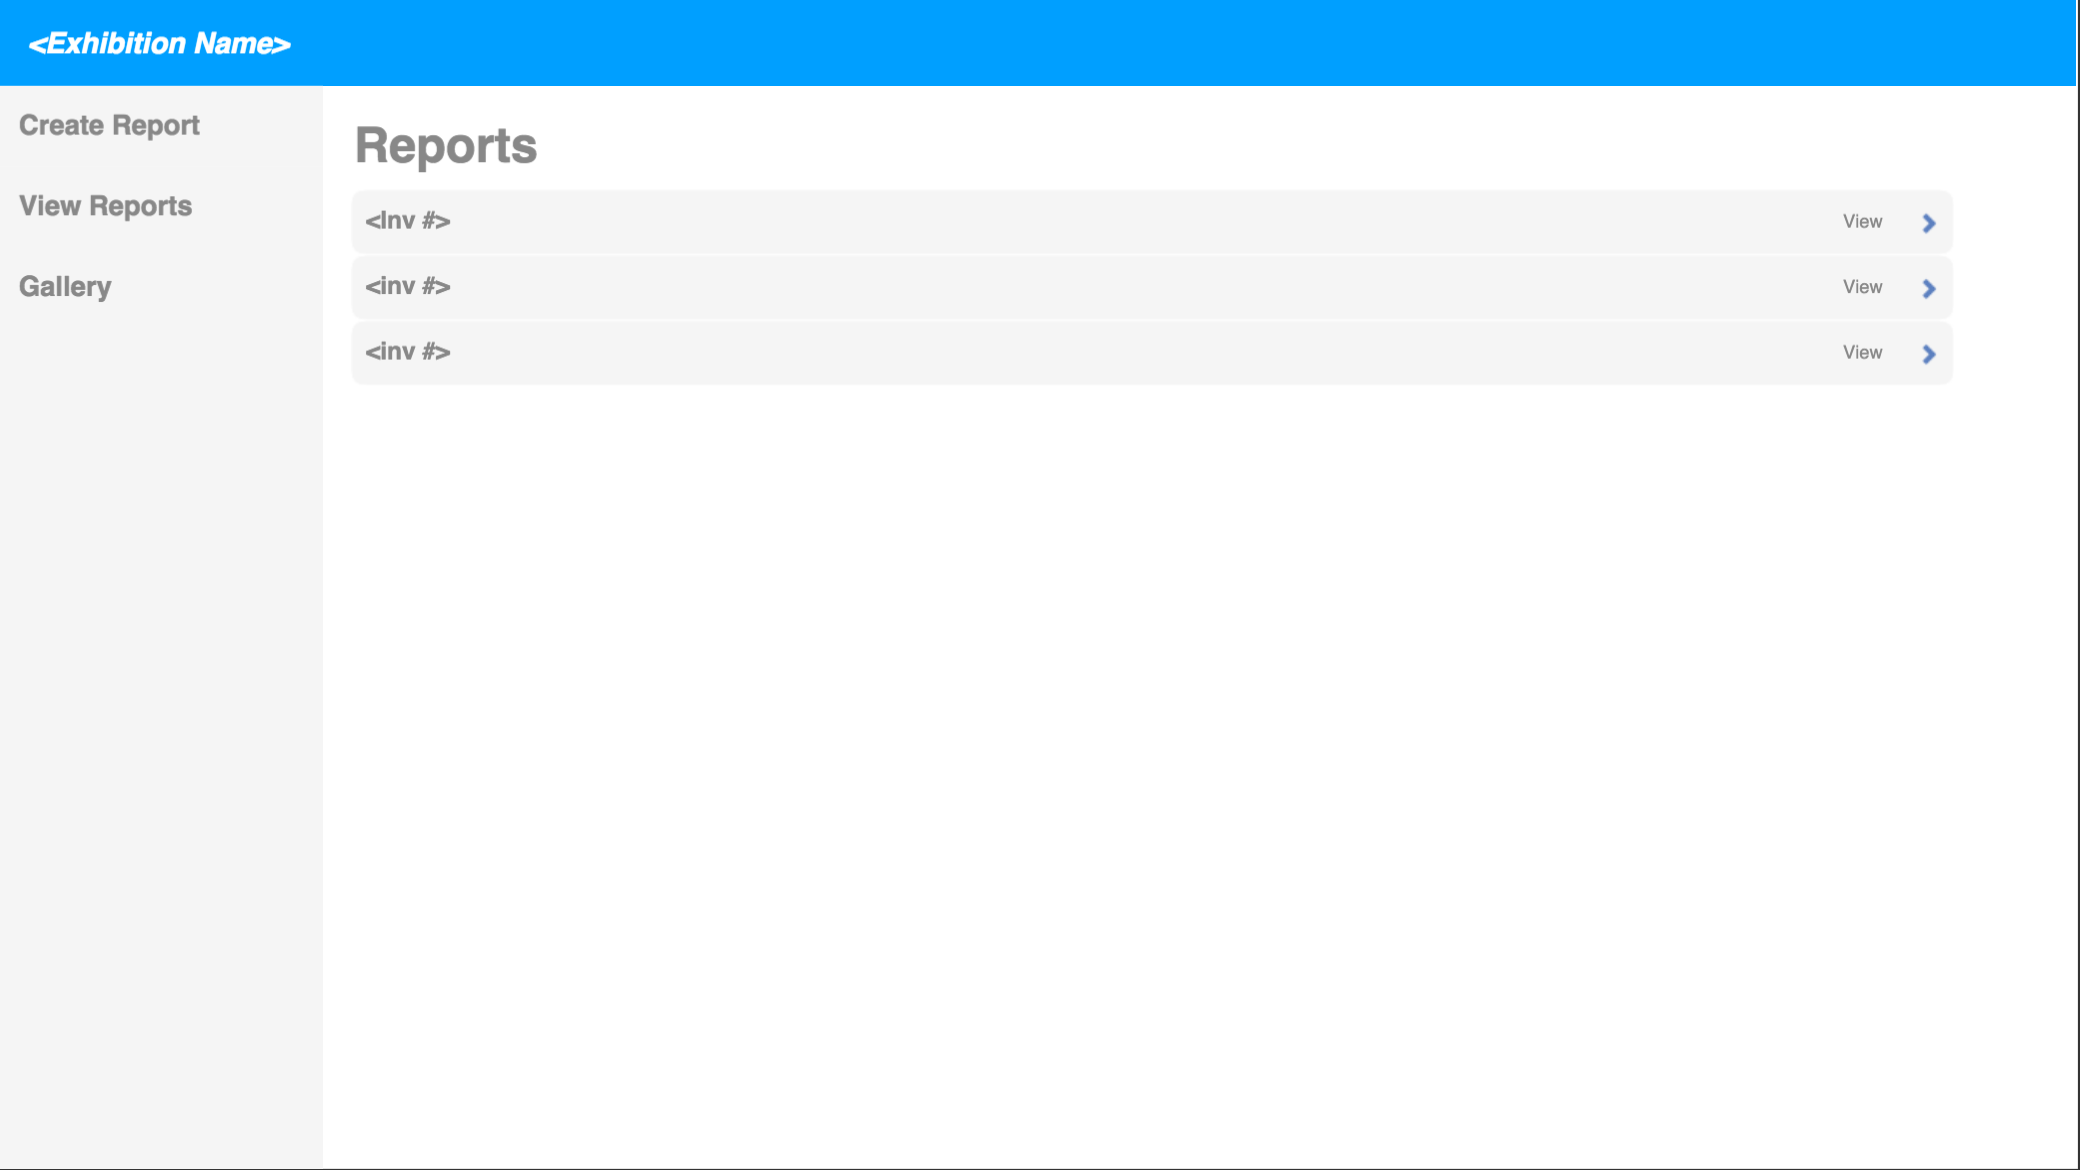
\includegraphics[scale=0.5]{mockup3.png}
\end{figure}
\begin{figure}
  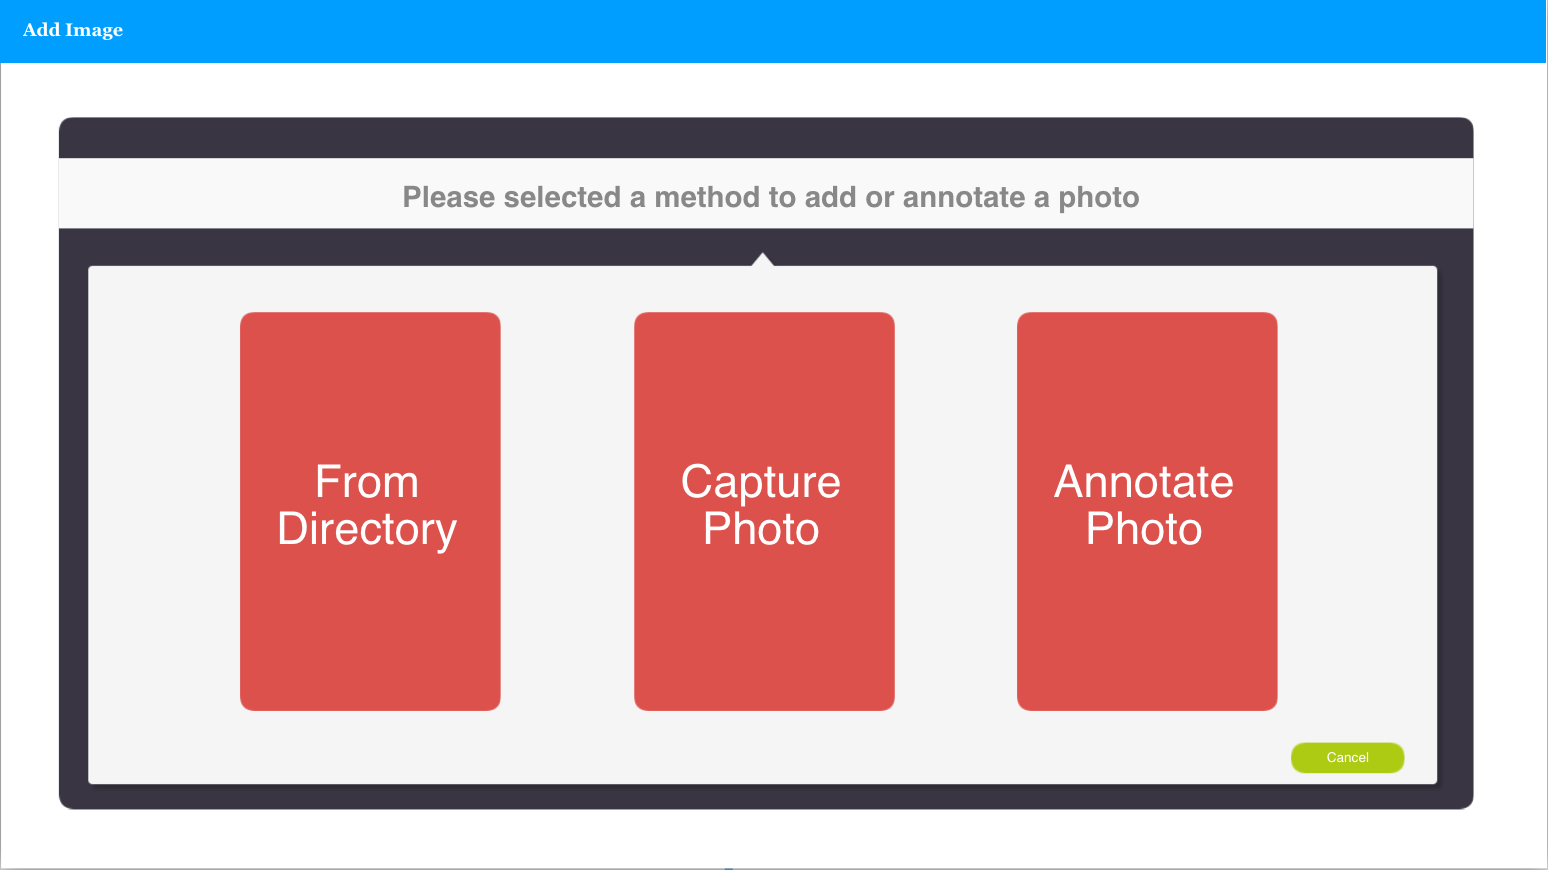
\includegraphics[scale=0.5]{mockup4.png}
\end{figure}
\begin{figure}
  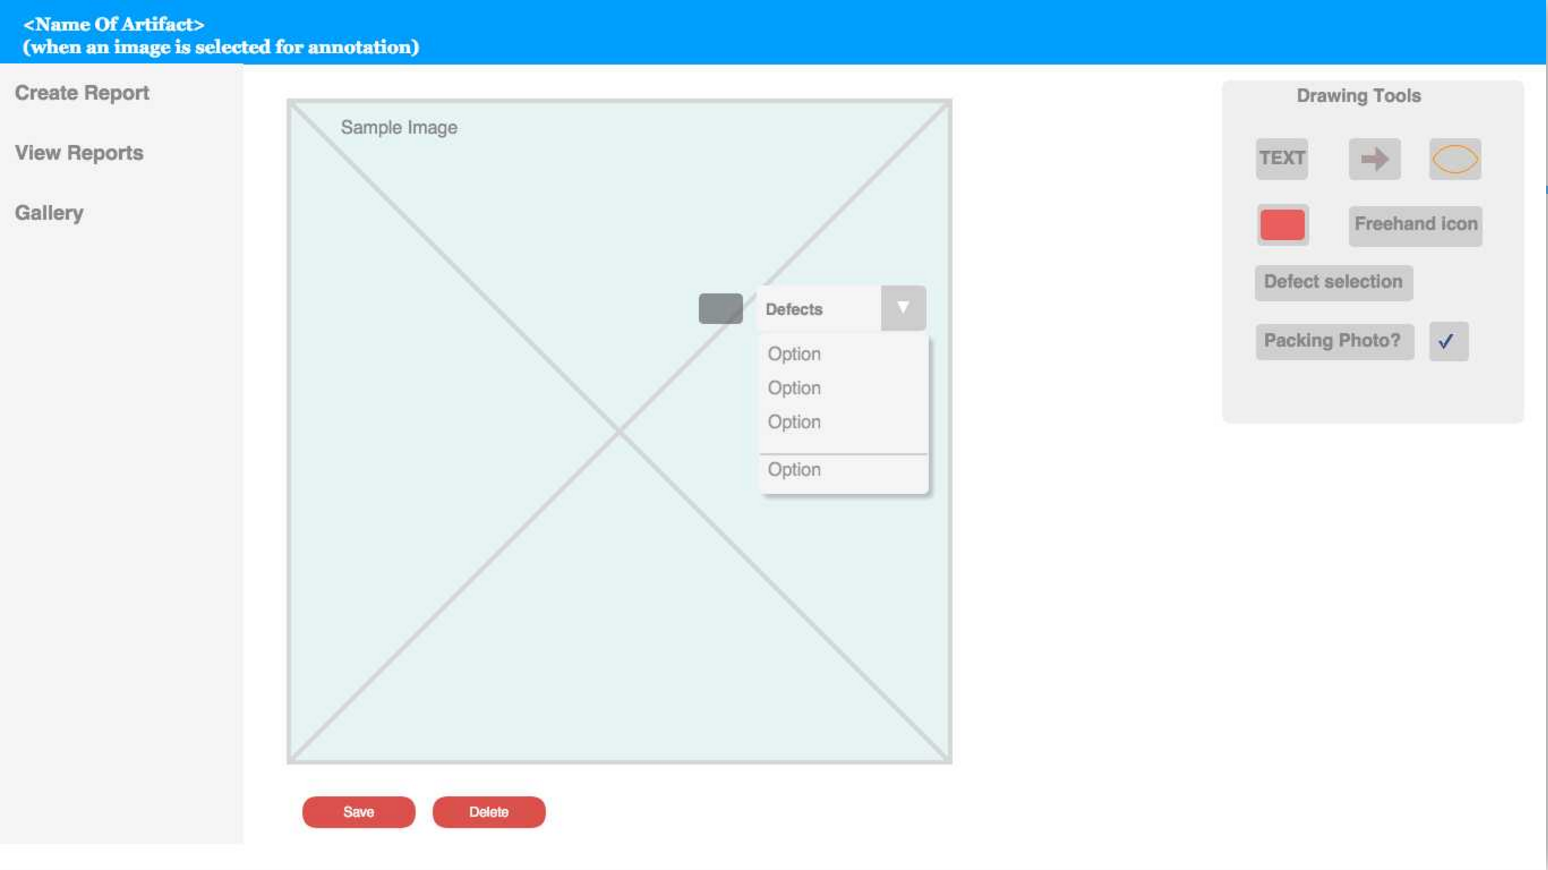
\includegraphics[scale=0.5]{mockup5.png}
\end{figure}
\begin{figure}
  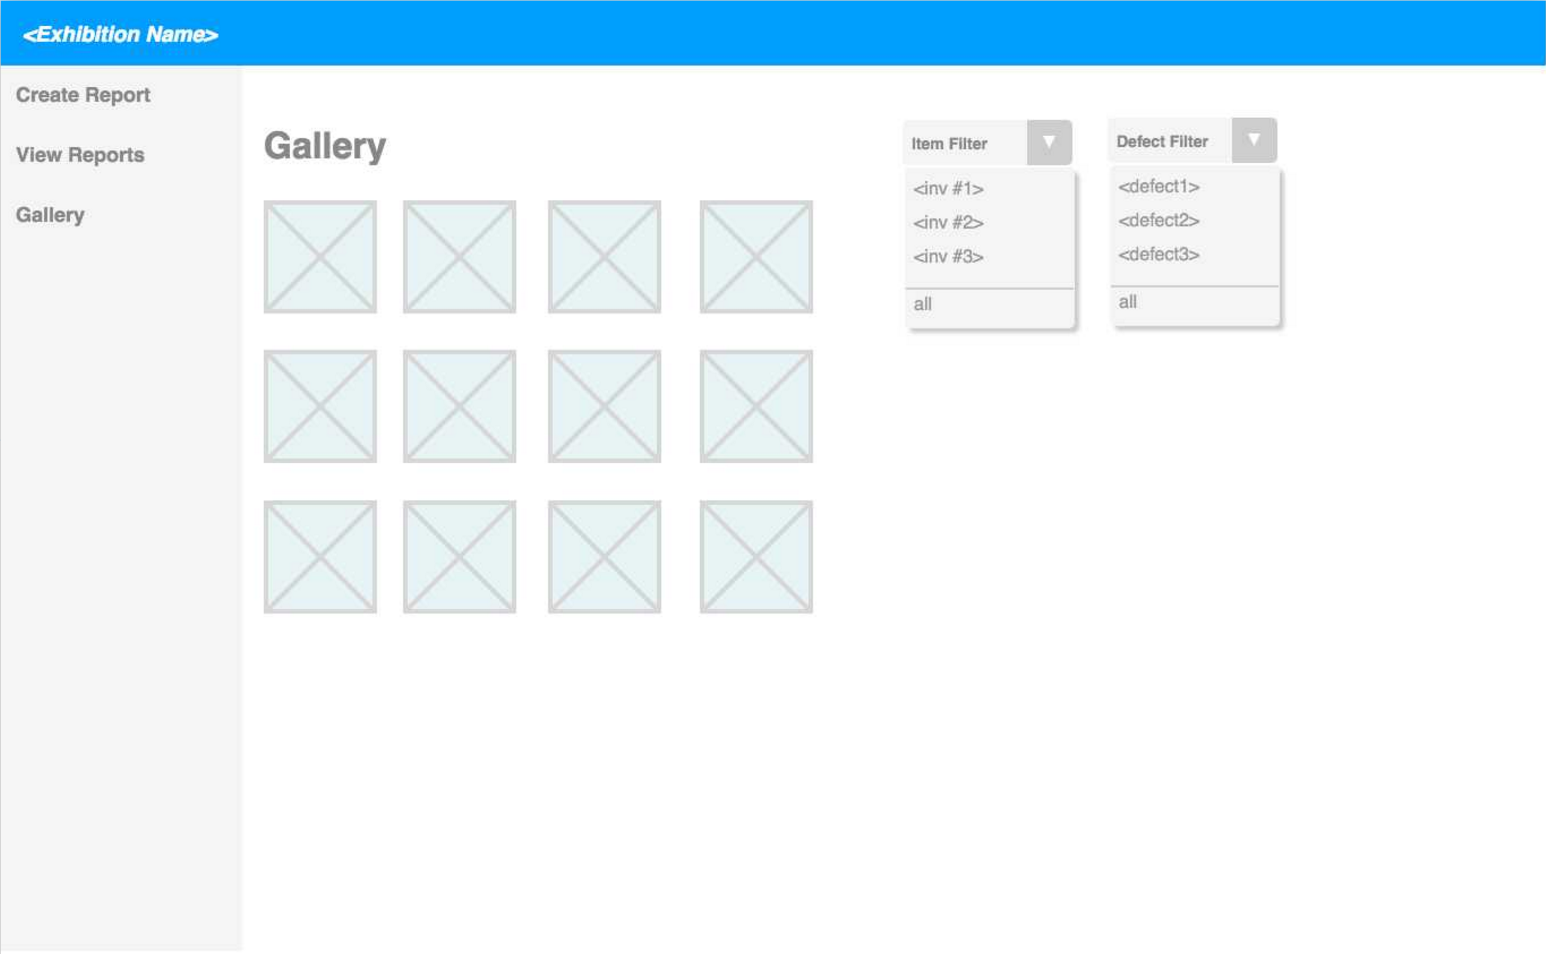
\includegraphics[scale=0.5]{mockup6.png}
\end{figure}
\end{document}